% Created 2013-10-01 Tue 13:47
\documentclass{beamer}
         \usepackage{color}
\usepackage{listings}
         \usepackage{natbib}
\usepackage{attachfile}
\usepackage{array}
\usetheme[numbers]{Dresden}
\setbeamercolor{structure}{fg=white}
\setbeamercolor*{palette primary}{fg=black,bg=white}
\setbeamercolor*{palette secondary}{use=structure,fg=white,bg=white}
\setbeamercolor*{palette tertiary}{use=structure,fg=white,bg=structure.fg!50!black}
\setbeamercolor*{palette quaternary}{fg=white,bg=black}
\setbeamercolor{item}{fg=red}
\setbeamercolor{subitem}{fg=orange}
\setbeamercolor*{sidebar}{use=structure,bg=structure.fg}
\setbeamercolor*{palette sidebar primary}{use=structure,fg=structure.fg!10}
\setbeamercolor*{palette sidebar secondary}{fg=white}
\setbeamercolor*{palette sidebar tertiary}{use=structure,fg=structure.fg!50}
\setbeamercolor*{palette sidebar quaternary}{fg=white}
\setbeamercolor*{titlelike}{parent=palette primary}
\setbeamercolor*{separation line}{}
\setbeamercolor*{fine separation line}{}
\setbeamertemplate{footline}[frame number]
\setbeamertemplate{navigation symbols}{}
\setbeamertemplate{subitem}[circle]
\newcommand{\sfootnote}[1]{\renewcommand{\thefootnote}{\fnsymbol{footnote}}\footnote{#1}\setcounter{footnote}{0}\renewcommand{\thefootnote}{\arabic{foot note}}}
\makeatletter\def\blfootnote{\xdef\@thefnmark{}\@footnotetext}\makeatother
\lstset{
keywordstyle=\color{blue},
commentstyle=\color{red},
stringstyle=\color[rgb]{0,.5,0},
basicstyle=\ttfamily\small,
columns=fullflexible,
breaklines=true,        % sets automatic line breaking
breakatwhitespace=false,    % sets if automatic breaks should only happen at whitespace
numbers=left,
numberstyle=\ttfamily\tiny\color{gray},
stepnumber=1,
numbersep=10pt,
backgroundcolor=\color{white},
tabsize=4,
showspaces=false,
showstringspaces=false,
xleftmargin=.23in,
frame=single,
basewidth={0.5em,0.4em}
}
\RequirePackage{fancyvrb}
\DefineVerbatimEnvironment{verbatim}{Verbatim}{fontsize=\small,formatcom = {\color[rgb]{0.5,0,0}}}
\itemsep2pt
\usetheme{default}
\author{Superman}
\date{\today}
\title{Power presentation}
\hypersetup{
  pdfkeywords={},
  pdfsubject={},
  pdfcreator={Emacs 24.3.1 (Org mode 8.0.7)}}
\begin{document}

\maketitle
\section{Section 1}
\label{sec-1}
\subsection{subSection 1}
\label{sec-1-1}
\begin{frame}[label=sec-1-1-1]{Slide 1}
\begin{itemize}
\item item 1
\item item 2
\item item 3
\end{itemize}
\end{frame}
\begin{frame}[fragile,label=sec-1-1-2]{Slide 2}
 \lstset{basicstyle=\small\tt,numbers=left,language=Lisp}
\begin{lstlisting}
M-j to export to latex and start latexmk
C-u M-j to debug
\end{lstlisting}
\end{frame}
\begin{frame}[label=sec-1-1-3]{Slide 3}
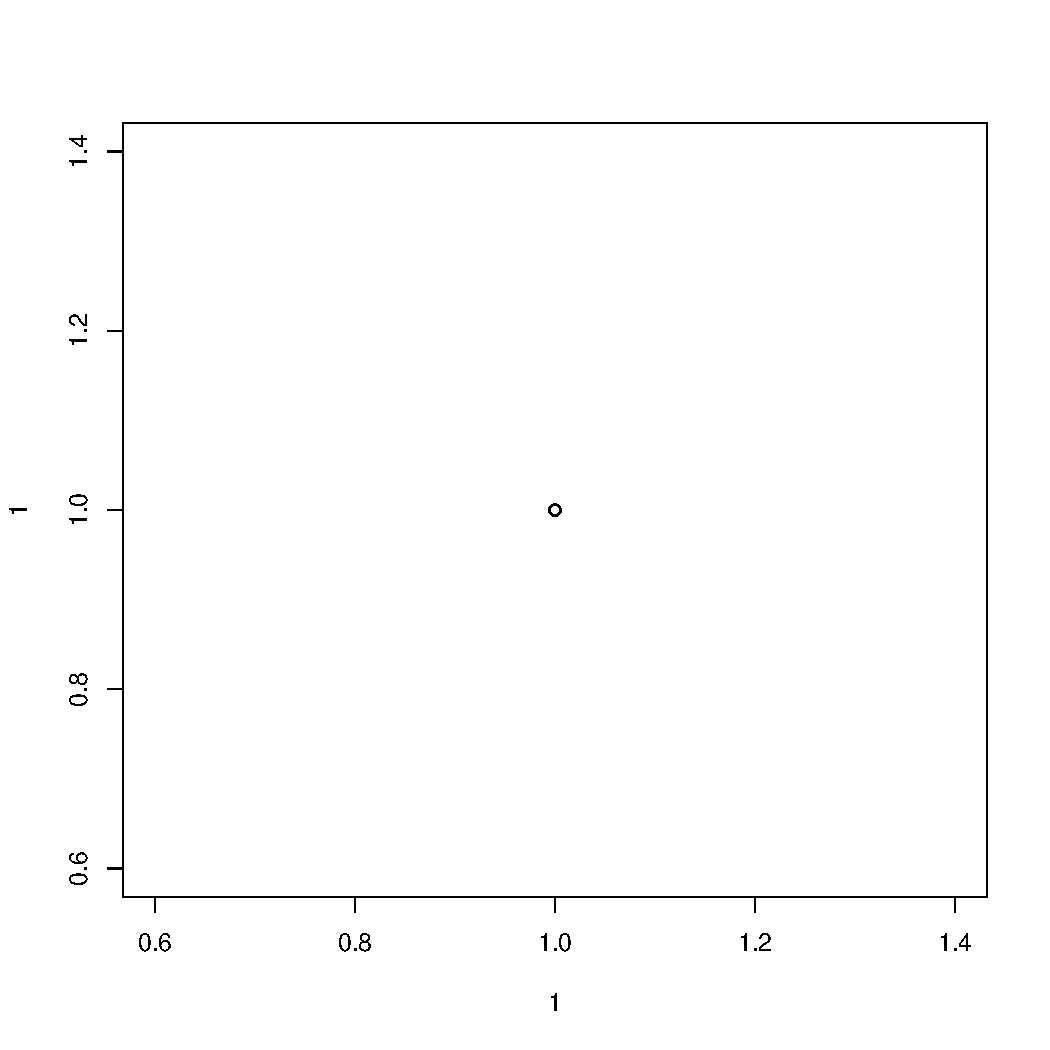
\includegraphics[width=.7\textwidth]{/home/ifsv/grb615/emacs-genome/genes/SuperMan/projects/Kal-El/test-graph.pdf}
\end{frame}
\begin{frame}[label=sec-1-1-4]{Slide 4}
\begin{columns}
\begin{column}{0.5\textwidth}
\begin{block}{A block in a column}

\end{block}
\end{column}
\begin{column}{0.5\textwidth}
Some text, the headline above is ignored

\end{column}
\end{columns}
\end{frame}
% Emacs 24.3.1 (Org mode 8.0.7)
\end{document}